\chapter{Results}
\label{Chapter3}
\section{Baseline models}
The simplest model for the gust factor is to guess the average gust factor for all available observations, i.e. use no variables from the training data. A slightly better model is obtained by using the wind speed as a training feature, either through regression or NN training. The MAPEs for the constructed base models are shown in Table \ref{table:baseline_models}. The ws$_{15}$ model was obtained with NN training but regression produces an almost identical result.

\begin{table}[h]
  \caption[MAPE for baseline models]{MAPE for several lower limits on the reanalysis 15 m wind speed ($ws_{15}$). Note that the ws$_{15}$ model was only evaluated for the 10 m/s lower bound.}
    \label{table:baseline_models}
    \centering
    \begin{tabular}{lcc}
        \toprule
        Wind speed & \multicolumn{2}{c}{MAPE}\\ 
        limit $[m/s]$ & mean model & ws$_{15}$ model\\
        \midrule
        $\geq 0$ & 39.2\%  & \\
        $\geq 5$ & 28.1\%  & \\
        $\geq 10$ & 23.9\% & 17.2\%\\
        $\geq 15$ & 23.2\% & \\
        $\geq 20$ & 24.7\% & \\
        $\geq 25$ & 27.7\% & \\
        \bottomrule
    \end{tabular}
\end{table}

As the average wind speed increases, then the variability in gust as a percentage decreases \cite{mean_gust_HA_HO}. Therefore lower MAPE would be expected if the training data is restricted to higher wind speeds. This fact explains why several models were created for different lower bounds.

\section{Modeling for ws$_{\textbf{15}}$ above 10 m/s}
As noted in Chapter \ref{Chapter1}, it is more important to predict accurate gust factor when it is windy than when the weather is calm. Therefore, at first, the data is restricted to ws$_{15} \geq 10$ m/s. The first constructed model incorporates the features temperature, pressure and wind direction at 15 m height. This gives a moderately reduced MAPE of 16.7\% compared with 17.2\% for the baseline ws$_{15}$ model. When the next pair of features, station altitude and transformed wind direction, is included, the MAPE is reduced considerably, down to 13.8\%. The atmospheric stability indicators, Ri and $N^2$, add little to the model performance, contrary to what might have been expected. When the atmosphere is unstable, wind gusts from higher up might be expected. However, another considerable performance increase is observed when digital elevation model (DEM) information is included, down to a MAPE of 12.0\%. This represents over 30\% reduction in the MAPE from the ws$_{15}$ baseline model. Adding all height levels decreases the loss but very little, as seen in the last line of the table.

The second last model in the Table \ref{table:setsOfParams} will be referred to as the \textit{primary model} and the corresponding parameters as the \textit{primary parameter set}. The model immediately before that is the \textit{secondary model}. In some cases the terminology ``primary parameter set with and without DEM'' will be used to refer to the parameter sets of these models.

\begin{table}[h]
  \caption[Model results for different sets of parameters.]{Models defined by a selection of parameter sets, with increasing complexity. The table shows decreasing MAPE as more variables are added.}
    \label{table:setsOfParams}
    \centering
    \begin{tabular}{lc}
        \toprule
        Model variables & MAPE\\
        \midrule
        $[\,]$ Baseline & 23.9\%\\
        $[ws_{15}]$ Baseline & 17.2\%\\
        $[ws_{15}, t_{15}, p_{15}, wd_{15}]$ & 16.7\% \\
        $[ws_{15}, t_{15}, p_{15}, wd_{15}, \text{altitude}, twd]$ & 13.8\% \\
        $[ws_{15}, t_{15}, p_{15}, wd_{15}, \text{altitude}, twd, N^2, Ri]$* & 13.7\%\\
        $[ws_{15}, t_{15}, p_{15}, wd_{15}, \text{altitude}, twd, N^2, Ri]$ + DEM** & 12.0\%\\
        $[ws_{15,250,500}, t_{15,250,500}, p_{15,250,500}, wd_{15,250,500}, \text{altitude}, twd, N^2, Ri]$ & 12.0\% \\
        \bottomrule
        *\small{Secondary model}
        **\small{Primary model}
    \end{tabular}
\end{table}

\section{Modeling for various ws$_\textbf{15}$ lower bounds}
To assess how model performance depends on ws$_{15}$ lower bound, several models were trained using the primary variable set, with and without DEM. The results can be seen in Table \ref{table:results}. For this investigation comparison was only made with the constant baseline model. In all cases adding the DEM information is seen to increase the model performance. The reason for the difference between the 10 m/s lower bound results seen in Tables \ref{table:setsOfParams} and \ref{table:results} is that they were obtained with different training setups. 

\begin{table}[h]
  \caption[Model results for different wind speed limits]{MAPE for each ws$_{15}$ lower bound without and with landscape elevation data (DEM) in a 30° sector into the direction of the reanalysis wind. Adding DEM data reduces the error noticably. Note that the MAPE is worse for both the lower lower bounds and the higher ones, but better for the intermediate ones.}
    \label{table:results}
    \centering
    \begin{tabular}{lccc}
        \toprule
        Wind Speed & \multicolumn{3}{c}{MAPE} \\
        limit $[m/s]$ & Baseline & Without DEM & With DEM \\
        \midrule
        $\geq 0$ & 39.2\% & 19.2\% & 18.9\% \\
        $\geq 5$ & 28.1\% & 15.3\% & 14.9\%\\
        $\geq 10$ & 23.9\% & 13.3\% & 12.5\%\\
        $\geq 15$ & 23.2\% & 14.4\% & 11.9\%\\
        $\geq 20$ & 24.7\% & 15.7\% & 13.3\%\\
        $\geq 25$ & 27.7\% & 19.4\% & 17.3\%\\
        \bottomrule
    \end{tabular}
  \end{table}

\section{Results for specific locations}
In this section, the distribution of MAPE by station will be considered. For each station the primary model MAPE was computed using just the ws$_{15} \geq 10$ data for that station was calculated and the results are shown in Figure \ref{fig:errorMap}. The stations with low performance are all near mountains and often in fjords. The worst cases are in Vestfirðir and Austfirðir, and several bad stations are e.g. in Tröllaskagi and Snæfellsnes, and near Öræfajökull, Esja, Eyjafjallajökull. Table \ref{table:more_specific_sites} shows the primary model MAPE together with the constant baseline reference for a few selected stations.

Inland stations seem to have lower error. The worst performing station is Seljalandsdalur in Vestfirðir while the best performing station is Garðskagaviti at the tip of the Reykjanes peninsula. Evidently rugged landscape makes it difficult to estimate the gust factor accurately.

\begin{figure}[h]
    \centering
    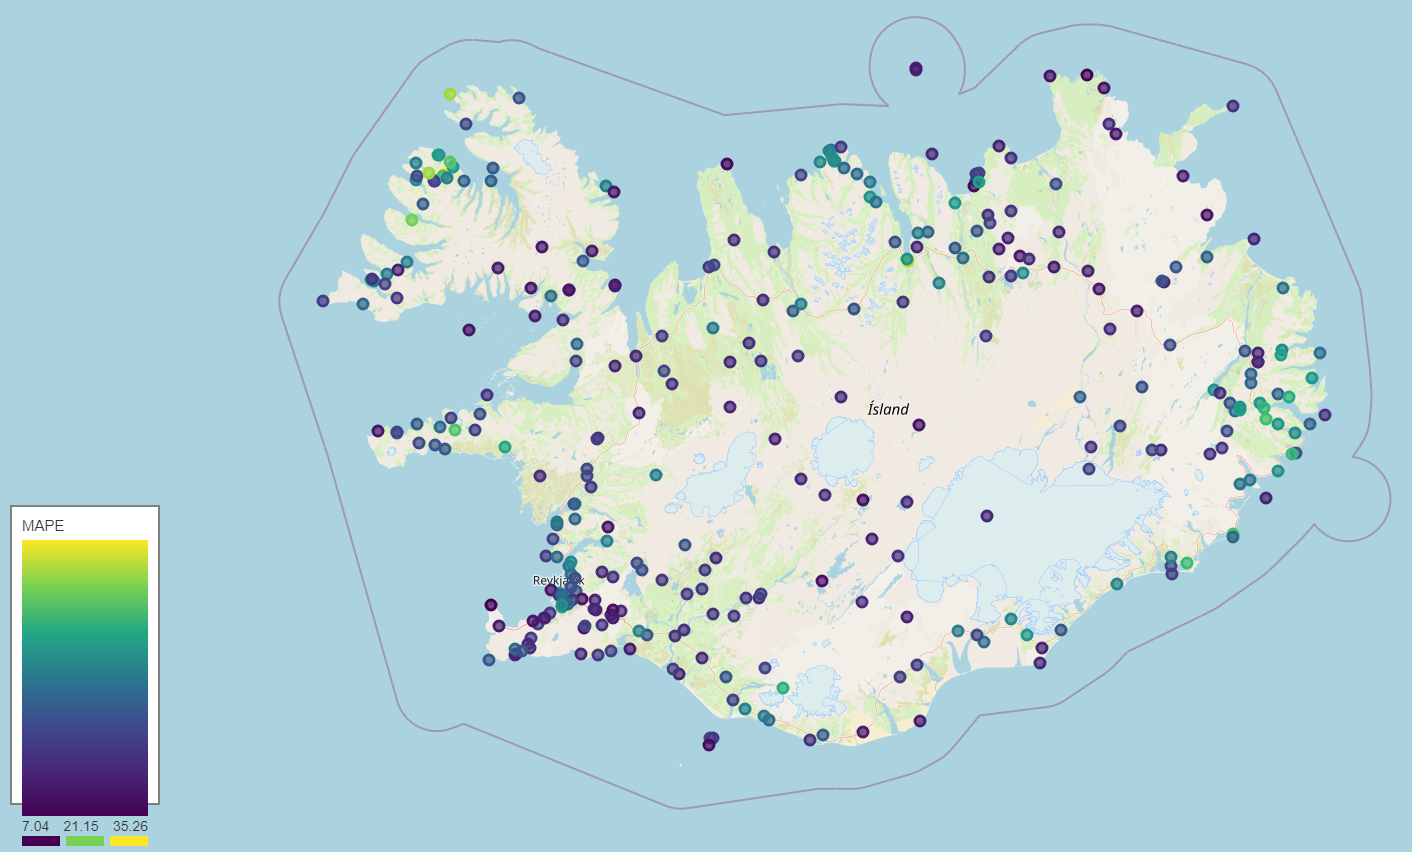
\includegraphics[scale = 0.5]{Figures/errorMap.png}
\caption[MAPE distribution by station]{Mean absolute percentage error (MAPE) at each station, shown as colored circles (dark blue = low error; yellow = high error). The lowest station error is about 7\% at Garðskagaviti and the highest about 35\% at Seljalandsdalur. The model uses a 10 m/s lower bound based on ws$_{15}$.}
\label{fig:errorMap}
\end{figure}

\begin{table}[h]
    \caption[Primary model MAPE by selected stations]{Constant baseline and primary model MAPE for a few selected stations. High MAPE values is seen in fjords near tall mountains in Austfirðir (Fáskrúðsfjörður and Seyðisfjörður), intermediate values at the foothills of mountains (Ingólfsfjall and Kjalarnes), and low values in flatter places (Sandskeið, Þrengsli).}
    \label{table:more_specific_sites}
    \centering
    \begin{tabular}{lcc}
        \toprule
        Station name & \multicolumn{2}{c}{MAPE}\\
         & Baseline & Model\\
        \midrule
        Fáskrúðsfjörður & 28.2\% & 21.8\%\\
        Ingólfsfjall & 30.0\% & 19.6\%\\
        Kjalarnes & 20.7\% & 13.5\% \\
        Sandskeið & 13.0\% & 10.2\%\\
        Seyðisfjörður & 32.1\% & 23.0\%\\
        Þjórsárdalur & 12.2\% & 11.4\%\\
        Þrengsli & 13.6\% & 11.3\%\\
        \bottomrule
    \end{tabular}
\end{table}

After examining the MAPE at each station individually, it is logical to try accounting for the station (or its location) in the model’s design. There are two ways to do this: To include the station location in the training data, and to train on subsets of the data, e.g. by station or groups of stations. Here the latter approach is considered. Results of an investigation for a few stations can be seen in Table \ref{table:specific_sites}. For many of the stations, the results are worse than expected, sometimes much worse, calling for further investigation.

\begin{table}[h]
  \caption[Model result by station]{MAPE for a few selected stations, for a model trained with the whole data set (general training), and for a model trained only with the data of the station itself (site training), with a lower bound of 10 m/s. This investigation was done in an earlier phase of the study, when $f$ instead of ws$_{15}$ was being used as the lower bound cut off, and that leads to some data leakage and a somewhat lower MAPE.}
    \label{table:specific_sites}
    \centering
    \begin{tabular}{lccc}
        \toprule
        Station name & n & \multicolumn{2}{c}{MAPE}\\
        & & General training & Site training\\
        \midrule
        Akrafjall & 43,000 & 18.6\% & 93.7\%\\
        Almannaskarð & 4,000 & 12.2\% & 86.7\%\\
        Ásgarðsfjall & 15,000 & 9.1\% & 9.4\%\\
        Jökulheimar & 17,000 & 7.7\% & 7.7\%\\
        Sandbúðir & 19,000 & 6.8\% & 6.4\%\\
        Stórholt & 35,000 & 7.1\% & 29.2\% \\
        Þúfuver & 20,000 & 6.4\% & 6.8\%\\
        \bottomrule
    \end{tabular}
\end{table}

\section{Results for wind speed intervals}
In addition to training for individual stations one can also try to train for individual wind speed intervals. Table \ref{table:closed_intervals} shows the results of training with the primary parameter set, with and without DEM. The table does not show noticeable improvement over the values in the last column in Table \ref{table:results}, in fact the two tables show quite similar results.

\begin{table}[h]
    \caption[Model result looking at closed wind speed intervals]{The MAPE results for different wind speed limit intervals. Here instead of training for all data above a certain threshold of wind speed, training is done only on data between two wind speeds. The percentage variance in gust factor as a function of wind speed increases with decreasing wind speed. Measured wind speed is used for the cutoff and thus have data leakage. These results should thus be somewhat comparable to the last column in Table \ref{table:results}}
    \label{table:closed_intervals}
    \centering
    \begin{tabular}{lcc}
        \toprule
        Interval &  \multicolumn{2}{c}{MAPE}\\
        $[m/s]$ & Without DEM & With DEM \\
        \midrule
        $[5, 10[$ & 17.1\% & 16.4\%\\
        $[10, 15[$ & 14.5\% & 13.0\%\\
        $[15, 20[$ & 15.0\% & 12.0\%\\
        $[20, 25[$ & 15.6 \% & 13.1\%\\
        $[25, 30[$ & 18.4\% & 19.0\%\\
        \bottomrule
    \end{tabular}
\end{table}

\section{Feature importance with Shapley values}
In this section Shapley values (see section \ref{sec:methodology} and \ref{sec:layout}) for the features of the secondary parameter set will be considered. Each feature value in each data row will contribute some share in the final prediction of an NN model, that can be computed by shifting the respective value and observe the change in the model output. This procedure is illustrated in Figure \ref{fig:ShapleyWaterfall}.

\begin{figure}[h]
  \centering
  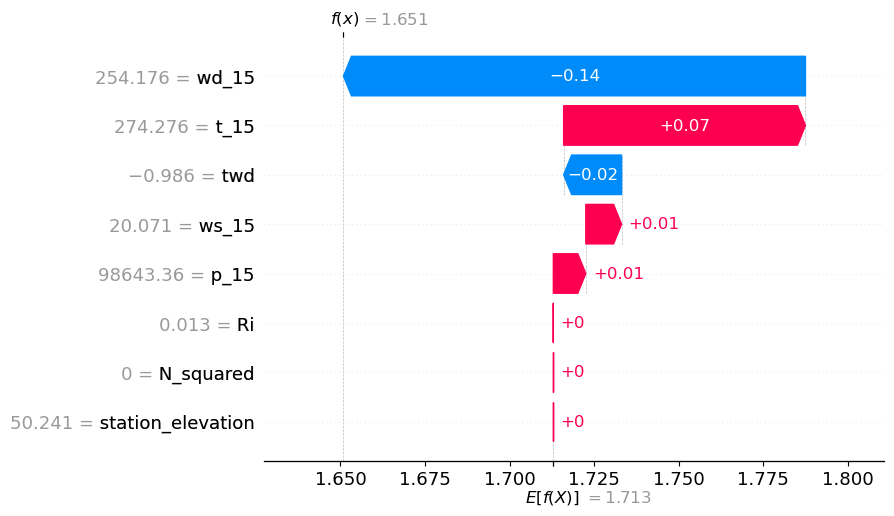
\includegraphics[scale = 0.6]{Figures/shap_plots/waterfall_plot.png}
  \caption[Shapley contributions for a single observation]{Shapley contributions for a single data row. The figure shows an example of the individual values contributing to a Shapley summary plot. Each point in a summary plot corresponds to one such instance. Several values with the same SHAP value will result in a thicker bulge in the summary. In this specific instance the wind direction ($wd_{15}$) has the highest negative contribution and the temperature has the highest positive contribution. The last three features contribute nothing.}
  \label{fig:ShapleyWaterfall}
\end{figure}

\subsection{Shapley summary plots for all stations}

Figure \ref{fig:ShapleySummary} provides a Shapley summary plot showing the contribution of each feature in the set. Computation of these values is expensive so subset of data is used ($\sim$1000 randomly selected data rows). There is an obvious outlier in the figure, making it difficult to assess the distribution. A second Shapley summary was computed with more data rows ($\sim$10000) and outliers excluded, see the lower panel of the figure. Note that it is not feasible to include the DEM data in this analysis, as they contain far too many variables.

Looking specifically at the lower panel in Figure \ref{fig:ShapleySummary}, the station elevation (altitude) is the most influential and the Richardson number's influence is very low, with the other features falling in between. For most features the Shapley values are bunch up around 0, while the station elevation, and to some extent ws$_{15}$ have a wider distribution. Station altitude/elevation seems to have a wide flat part between –0.1 and 0.1. Overall, the values seem to have a longer right tail. This is expected as gust factors are positive ($\sim$1.2 to 2). Notice also that Ri has virtually no contribution and could safely be removed from the model.

The coloring of the points in the displayed distributions show the corresponding feature values. For example, in the lower panel of Figure \ref{figure:ShapleySummary}, high station altitude/elevation corresponds to negative contribution and vice versa, and same for $p_{15}$. For ws$_{15}$ and $t_{15}$ the relationship is opposite, with high feature values corresponding to positive contribution. When the coloring is more mixed the contribution of the feature is more mixed. For example, high twd might have a positve contribution at some locations but negative elsewhere.

\begin{figure}
  \centering
  \begin{subfigure}{0.9\textwidth}
    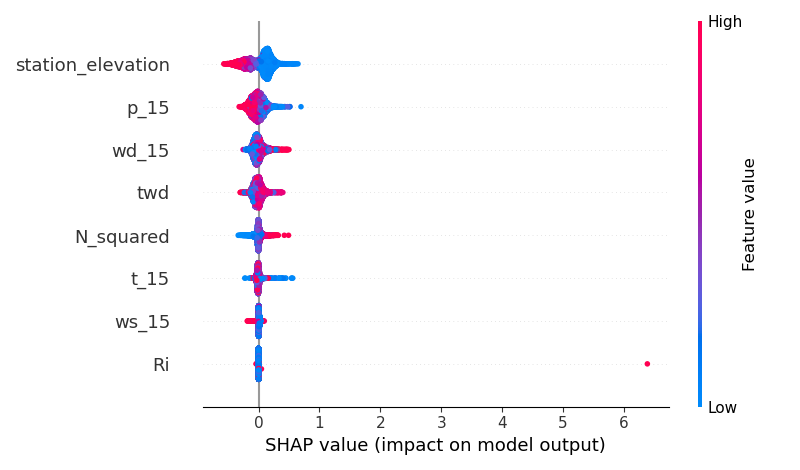
\includegraphics[width=\textwidth]{Figures/shap_plots/summary_plot.png}
  \end{subfigure}
  \vspace{0.5cm}
  \begin{subfigure}{0.9\textwidth}
    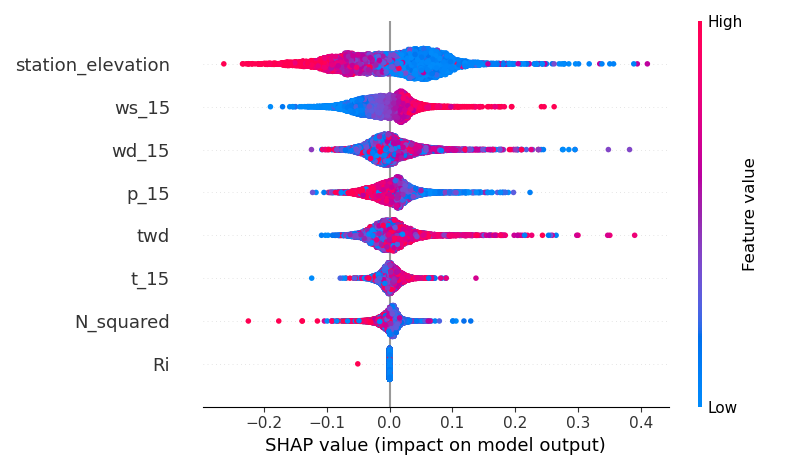
\includegraphics[width=\textwidth]{Figures/shap_plots/summary_plot_190924_.png}
  \end{subfigure}
  \caption[Shapley summary plots]{Shapley summary plots showing feature importance for the secondary model described in Table \ref{table:setsOfParams}, with randomly chosen subsets of the data. SHAP values with high absolute value indicate high contribution of the corresponding feature. Coloring shows the respective feature value, blue for low and red for high. For example high station altitude/elevation corresponds to negative contribution and vice versa, and for ws$_{15}$ the relationship is opposite, with high feature values corresponding to positive contribution. It can be seen that generally multiple factors influence the prediction, with the station elevation being highly influential. There is one outlier in the upper panel, for the Richardson number, which otherwise has very little influence. The upper panel is based on $\sim$1000 data rows. The lower panel is based on more data rows ($\sim$10000), and furthermore, outliers have been removed there to make the plot more legible.}
  \label{fig:ShapleySummary}
\end{figure}

Figure \ref{fig:ShapleySummary3} in Appendix A shows a Shapley summary plot for all the data rows. However this plot is detrimentally affected outliers.

\subsection{Shapley summary plots for individual stations}
It can also be informative to look at summary plots for individual stations. In this subsection two such examples are considered, for Akrafjall and Keflavíkurflugvöllur. It is noteworthy to see that the constant value of a stations altitude produces quite different contributions to the predictions, presumable because of diffent interactions with other features. For (very) simple models, such as linear regression without cross terms, this would not happen.

\begin{figure}
    \centering
    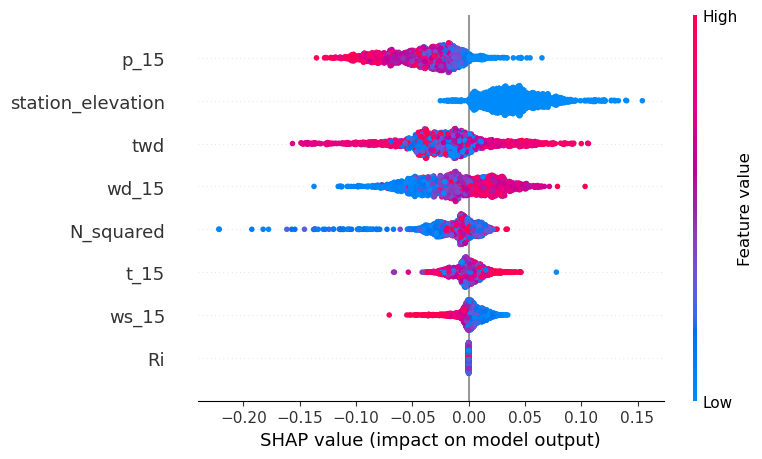
\includegraphics[scale = 0.6]{Figures/shap_plots/summary_plot_1350.png}
    \caption[Summary feature importance of a neural network only looking at AWS at Keflavíkurflugvöllur.]{Feature importance of a neural network with model architecture as described in Table \ref{table:gridSearchHyperparameters} and data as described in Table \ref{table:trainDataExample}. This plot only looks at datapoints from Keflavíkurflugvöllur. This seems to show the same distribution as previous summary plots. Station elevation is influential and Richardson number has no impact.}
    \label{fig:ShapleySummaryKeflavikurflugvollur}
\end{figure}

\begin{figure}
    \centering
    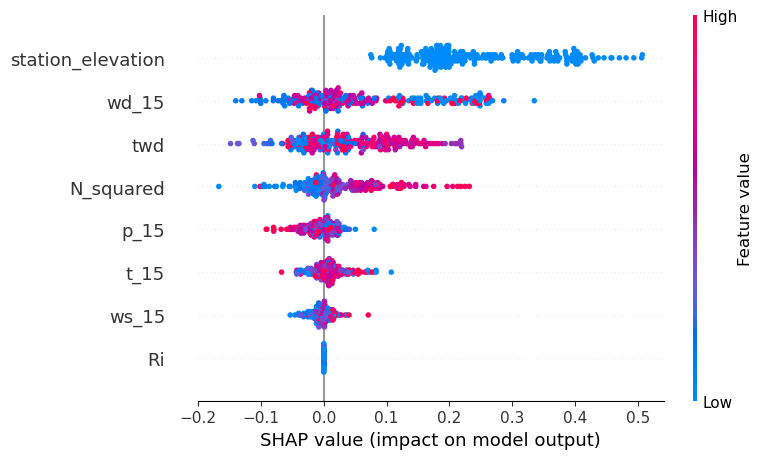
\includegraphics[scale = 0.6]{Figures/shap_plots/summary_plot_35553.png}
    \caption[Summary feature importance of a neural network only looking at AWS at Almannaskarð.]{Feature importance of a neural network with model architecture as described in Table \ref{table:gridSearchHyperparameters} and data as described in Table \ref{table:trainDataExample}. This plot only looks at datapoints from Almannaskarð. This seems to show the same distribution as previous summary plots. Station elevation is influential and Richardson number has no impact.}
    \label{fig:ShapleySummaryAlmannaskarð}
\end{figure}

\begin{figure}
    \centering
    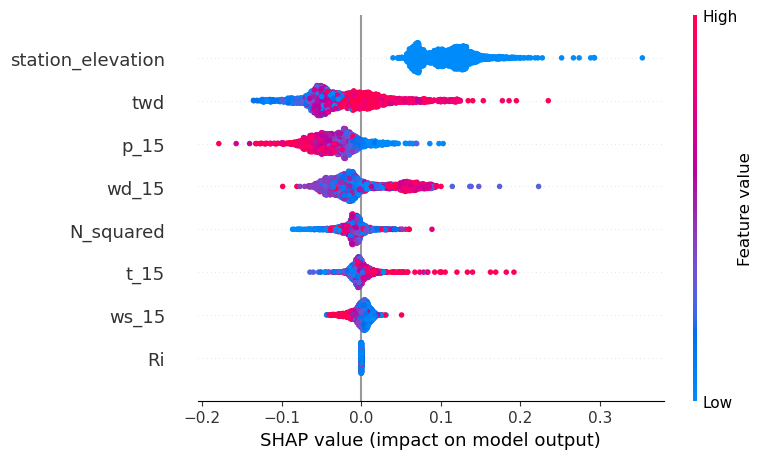
\includegraphics[scale = 0.6]{Figures/shap_plots/summary_plot_31572.png}
    \caption[Summary feature importance of a neural network only looking at AWS at Akrafjall.]{Feature importance of a neural network with model architecture as described in Table \ref{table:gridSearchHyperparameters} and data as described in Table \ref{table:trainDataExample}. This plot only looks at datapoints from Akrafjall. This seems to show the same distribution as previous summary plots. Station elevation is influential and Richardson number has no impact.}
    \label{fig:ShapleySummaryAkrafjall}
\end{figure}

Further examples of Shapley summary plots for individual stations may be found in Appendix A.

It is important to note that Shapley summary plot analysis assumes feature independence, because only one feature at a time is changed \cite{Salih_2024}. This might explain why the impact of the Richardson number is so low. Both the squared Brunt–Väisälä frequency and the Richardson number are measures of atmospheric stability and partly depend on the same variables, i.e. pressure and temperature at different height levels, as seen in Equations (\ref{eqn:Ri}) and (\ref{eqn:N}). Shapley tries to assign contribution values for each feature for each observation, but how the contribution should be distributed between the two features is not clear. If the Brunt–Väisälä would be excluded from the data, the impact of the Richardson number would likely increase.

Another point to note is that the features are ordered by their impact. The station altitude is the most impactful for all the plots except Keflavíkurflugvöllur (Figure \ref{fig:ShapleySummaryKeflavikurflugvollur}), but the ordering of other variables changes. Looking at the lower panel of Figure \ref{fig:ShapleySummary}, the wind speed is the second most important feature. This is reversed in Figure \ref{fig:ShapleySummaryAlmannaskarð}. This is not unexpected as the Almannaskarð station was specifically selected as a station with high MAE between observed and reanalysis wind speed (Table \ref{table:station_mae_distribution}. Another station with high MAE is Akrafjall, with a Shapley summary plot in Figure \ref{fig:ShapleySummaryAkrafjall}).

What is interesting is that the reanalysis wind speed is also of low impact at stations like Keflavíkurflugvöllur, as shown in Figure \ref{fig:ShapleySummaryKeflavikurflugvollur} which had the second lowest MAE difference between measured wind speed and reanalysis wind speed (see Table \ref{table:station_mae_distribution}). Another such station, in fact the one with the lowest MAE, is Háahlíð in Reykjavík. The Shapley summary plot for this station is shown in Appendix A (\ref{fig:ShapleySummaryHaahlid}).

\section{CARRA wind gust}
% In 4.3, add commas in first sentence
% Later in 4.3, add "that" before "they"
% Table 4.3, change higher to worse, add: but better for the intermediate ones

The CARRA dataset provides no gust values in its analysis component but does include 10 m wind gust in the forecast. With a shortest lead time of one hour and given that a model of the gust factor is to be constructed, it stands to reason to incorporate the one-hour forecast CARRA gust factor, computed as:
\begin{equation*}
\text{CARRA gust factor} = \dfrac
{\text{1 hr forecast 10 m wind gust}}
{\text{1 hr forecast 10 m wind speed}}
\end{equation*}
into the modelling, as a proxy for a reanalysis wind gust.

One issue with the CARRA gust factor is that it is not available for several time points including the period after the middle of 2022, whereas the CARRA reanalysis data used in this study extends through 2023, making it somewhat involved to assess its predictive power. Two investigations were carried out. First, the reduction in MAPE resulting from the addition of the CARRA gust factor to the baseline ws$_{15}$, secondary, and primary NN models of Section 4.2 was assessed, using only data with CARRA gust available. The results of this comparison are shown in Table \ref{table:carra_gust}

\begin{table}[h]
  \centering
  \caption[Results adding CARRA gust factor]{Results of adding the CARRA gust factor as a variable in selected models from Sections 4.2 and 4.3.}
  \label{table:carra_gust}
  \begin{tabular}{lcc}
    \toprule
    & \multicolumn{2}{c}{MAPE\qquad\qquad} \\
    Model & Unaltered & With CARRA gust factor \\
    \midrule
    Baseline ws$_{15}$ model & 17.0\% & 16.7\% \\
    Secondary model           & 13.3\% & 13.2\% \\
    Primary model             & 12.5\% & 12.4\% \\
    \bottomrule
  \end{tabular}
\end{table}

The causes of the differences between the numbers in Table \ref{table:carra_gust} and those of Tables 4.2 and 4.3 could be different time period and/or unlike training setup.

Second, three simple linear regression models were constructed involving ws$_{15}$ and the CARRA gust factor, using available data with ws$_{15} \geq 10$ m/s. The results are shown in Table \ref{table:carra_gust_regression}.

\begin{table}[h]
  \centering
  \caption[Regression MAPE with and without CARRA gust factor]{Mean absolute percentage error (MAPE) for regression models using the CARRA gust factor, ws$_{15}$, and both combined.}
  \label{table:carra_gust_regression}
  \begin{tabular}{lc}
    \toprule
    Model                         & MAPE   \\
    \midrule
    ws$_{15}$                     & 17.03\% \\
    CARRA–gf                      & 16.81\% \\
    CARRA–gf + ws$_{15}$          & 16.80\% \\
    \bottomrule
  \end{tabular}
\end{table}

Finally, using the raw CARRA gust factor without any modelling gave MAPE = 18.14\%.

The conclusion that can be drawn from this investigation is that there is a modest information in the CARRA wind gust forecast, potentiially reducing model MAPE by 0.1 to 0.3 percentage points. This reduction is however quite small compared with the overall MAPE reduction of $\sim$5 percentage points seen in Table 4.2 when all available variables are added.
